\vspace*{\subsecspace}
\section{Related Work}
\label{sec:related}


\sysname builds upon a large body of prior work on running scientific computing applications on the cloud, and the various facets of transient cloud computing.  

\vspace*{\subsecspace}
\subsection{Cloud Computing For Science}
Running scientific applications on the cloud introduces many tradeoffs compared to conventional HPC clusters, along the dimensions of performance, cost, scalability, convenience, and reproducability.
These tradeoffs are explored in~\cite{iosup_performance_2011, zhai_cloud_2011, marathe2013comparative, galante_analysis_2016, benedictis_cloud-aware_2014}.
In general, clouds can provide increased elasticity, lower waiting times, and more choices in resource allocation that can be tailored to the application.
The cloud resource model is also present in platforms like nanoHUB~\cite{nanohub}, that provide easy execution and dissemination of nanotechnology simulation applications.
%such as Ref.~\cite{kadupitiya2017}.
Outside of the bags of jobs execution model, price optimizations for scientific workflows in the cloud is discussed in~\cite{gari_learning_2019}. 
While bags of tasks~\cite{varshney_autobot_2019} are often used for parallel applications, \sysname is the first to use of the bags of \emph{jobs} abstraction for efficient and effective use of transient servers. 

%\subsubsection{Bags of Jobs}
\vspace*{\subsecspace}
\subsection{Transient Cloud Computing}

%The low cost of transient cloud servers has made them very appealing, inspite of their preemptible nature, and their efficient and effective use has been a significant amount of research~\cite{prateek-thesis}. 
The challenges posed by Amazon EC2 spot instances, the first transient cloud servers, have received significant attention from both researchers and industry~\cite{spotinst}.
Since spot instances are significantly cheaper than the equivalent on-demand servers, they are attractive for running preemption and delay tolerant batch jobs~\cite{spoton, jain14demand, yi2010reducing, conductor, liu-spot, spot-run, dubois2016optispot}.
A crucial component of EC2 spot instances is their dynamic auction-based pricing, and choosing the ``right'' bid price to minimize cost and performance degradation is the focus of much of past work on transient computing~\cite{bidding4,mihailescu2012impact,bidding7,bidding1,bidding8,bidding3,bidding6,bid-cloud,bidding5,wolski_probabilistic_2017, guo_bidding_2015}.
However, as explained in Section~\ref{subsec:need-for-empirical}, it remains to be seen how Amazon's recent change~\cite{bid-change} in the preemption model of spot instances affects prior work.


On the other hand, the effective use of transient resources provided by other cloud providers such as Google, Microsoft, Packet, and Alibaba largely remains unexplored. 
Ours is the first work that studies the preemption characteristics and addresses the challenges involved in running large-scale applications on the Google Preemptible VMs, and provides insights on and leverages the unique preemption dynamics, as explained in Section~\ref{sec:preemption-dynamics}.

\vspace*{\subsecspace}
\subsubsection{Preemption Mitigation}
Effective use of transient servers usually entails the use of fault-tolerance techniques such as checkpointing~\cite{flint}, migration~\cite{spotcheck}, and replication.
In the context of HPC workloads,\cite{marathe2014exploiting,gong_monetary_2015,xiang_spotmpi:_2011} develop checkpointing and bidding strategies for MPI applications running on EC2 spot instances, based on older spot pricing data and model.
A comprehensive survey on periodic checkpointing for HPC applications can be found in~\cite{dongarra_fault_nodate}.  

By treating bags of jobs as an execution unit, allowing some jobs to fail, and using insights from preemption models, we show that it is possible to reduce the recomputation times to acceptable levels even without the  use of periodic  checkpointing that imposes additional deployment and performance overheads.
%The first step towards mitigating preemptions is understanding their characteristics. 
Our preemption model for Google preemptible VMs developed in Section~\ref{sec:preemption-dynamics} extends the classic Weibull-distribution based bathtub models~\cite{mudholkar1993exponentiated,crevecoeur1993model} by introducing exponential reclamation near the deadline and additional paramters that capture and explain the preemption dynamics. 

\vspace*{\subsecspace}
\subsubsection{Server Selection}

Optimized server selection is an important problem in cloud computing, and especially for transient servers because of the cost-performance-preemption tradeoff involved. 
Similar to \sysname, SpotOn~\cite{spoton} is also a batch computing service that selects servers based on job characteristics and failure rates of different EC2 spot VMs. However, it is restricted to individual, single-VM batch jobs, and its design is tied to EC2 spot instances.
The state of the art transient server selection involves the use of multiple types of VMs~\cite{exosphere}, and selecting a heterogeneous cluster can reduce the likelihood of mass concurrent preemptions.
However, since scientific computing applications are mostly synchronous, even a single failure affects the entire job, and heterogeneous clusters are not required, and are in fact, detrimental. 
Server selection is important even outside of preemptible VMs---developing bayesian optimization and application performance model based search for the ``best'' cloud VM is an active research area~\cite{alipourfard_cherrypick, yadwadkar_selecting_2017}. 

\begin{figure}[t]
  \centering 
       \vspace*{\myfigspace} 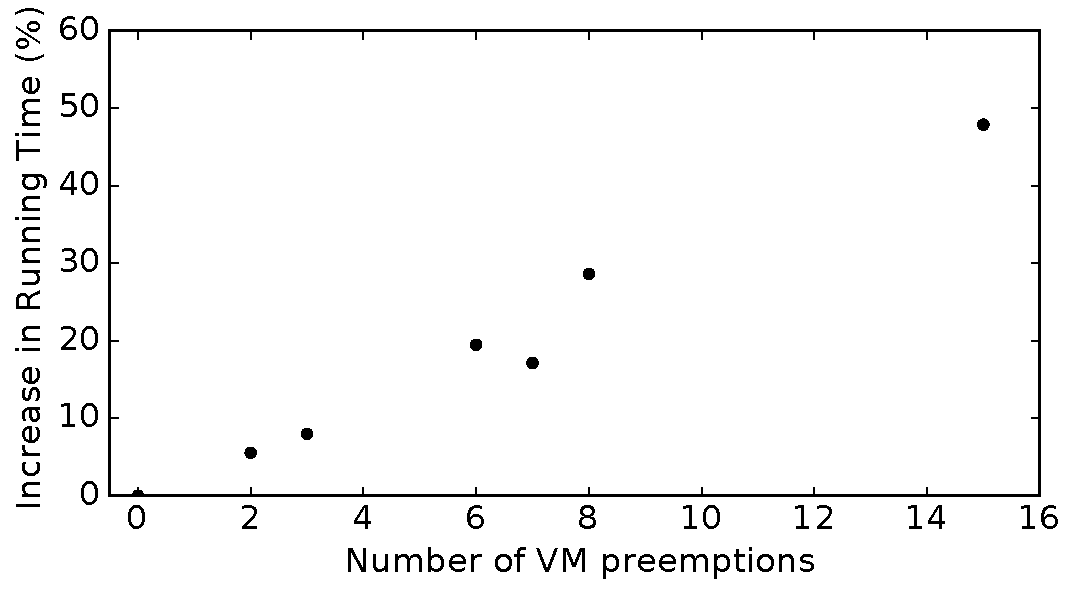
\includegraphics[width=0.22\textwidth]{../graphs/confin-fails-vs-time-relative.pdf}
      \vspace*{\myfigspace}
  \caption{The increase in running time due to preemptions is under 50\%, even when the number of preemptions is high.}
  \label{fig:fails-time}
        \vspace*{\myfigspace}
\end{figure}




\vspace*{\subsecspace}
%Parameter sweep aka bags of jobs ~\cite{casanova_heuristics_2000}

%But nothing for bags of jobs themselves.. 


% \subsubsection{Fault-tolerance}

% All the past work was on EC2 spot market with gang failures and independent markets~\cite{marathe2014exploiting, gong_monetary_2015}.
% However this assumption has now changed, and failures can happen anytime.
% Our failure model is more general, and applies to both cases.



% \cite{dongarra_fault_nodate} has a discussion of checkpointing frequency which is comprehensive. Replication is another way~\cite{walters_replication-based_2009}

% Non periodic checkpointing~\cite{bougeret_checkpointing_2011}


% \subsubsection{Failure Modeling}



% Crevecour etc. 



% \subsubsection{Server Selection}
% Exploring a large configuration space using bayesian optimization methods in CherryPick~\cite{alipourfard_cherrypick} and Metis~\cite{li2018metis}.

% Can also use Latin Hypercube sampling for parameter exploration?




%%% Local Variables:
%%% mode: latex
%%% TeX-master: "paper"
%%% End:
